\let\negmedspace\undefined
\let\negthickspace\undefined
\documentclass[journal]{IEEEtran}
\usepackage[a4paper, margin=10mm, onecolumn]{geometry}
\usepackage{lmodern} % Ensure lmodern is loaded for pdflatex
\usepackage{tfrupee} % Include tfrupee package

\setlength{\headheight}{1cm} % Set the height of the header box
\setlength{\headsep}{0mm}  % Set the distance between the header box and the top of the text

\usepackage{gvv-book}
\usepackage{gvv}
\usepackage{cite}
\usepackage{amsmath,amssymb,amsfonts,amsthm}
\usepackage{algorithmic}
\usepackage{graphicx}
\usepackage{float}
\usepackage{textcomp}
\usepackage{xcolor}
\usepackage{txfonts}
\usepackage{listings}
\usepackage{enumitem}
\usepackage{mathtools}
\usepackage{gensymb}
\usepackage{comment}
\usepackage[breaklinks=true]{hyperref}
\usepackage{tkz-euclide} 
\usepackage{listings}
% \usepackage{gvv}                                        
\def\inputGnumericTable{}                                 
\usepackage[latin1]{inputenc}                                
\usepackage{color}                                            
\usepackage{array}                                            
\usepackage{longtable}                                       
\usepackage{calc}                                             
\usepackage{multirow}                                         
\usepackage{hhline}                                           
\usepackage{ifthen}                                           
\usepackage{lscape}
\usepackage{tikz}
\usetikzlibrary{patterns}

\begin{document}

\bibliographystyle{IEEEtran}
\vspace{3cm}

\title{2.5.32}
\author{EE25BTECH11064 - Yojit Manral}

\maketitle
% \maketitle
% \newpage
% \bigskip
{\let\newpage\relax\maketitle}
\renewcommand{\thefigure}{\theenumi}
\renewcommand{\thetable}{\theenumi}
\setlength{\intextsep}{10pt} % Space between text and float

\textbf{Question:}\\
Show that the points $\brak{7,10}$, $\brak{-2,5}$ and $\brak{3,4}$ are vertices of an isosceles right triangle.\\

\textbf{Solution:}\\
\begin{table}[h!]    
  \centering
  \begin{tabular}[12pt]{ |c| c|}
    \hline
    \textbf{Points} & \textbf{Name}\\ 
    \hline
	\myvec{7\\10} & Point $\Vec{A}$ \\
    \hline 
	\myvec{-2\\5} & Point $\Vec{B}$\\
    \hline
	\myvec{3\\4} & Point $\Vec{C}$\\
    \hline
\end{tabular}
  \caption{List of Points}
  \label{Table_1}
\end{table}\\

$\rightarrow$ We have $\triangle$ABC with the given points. Then,

\begin{align}
    \norm{\vec{B} - \vec{A}}^2 = \myvec{-9 & -5}\myvec{-9\\-5} &= 106 \implies \norm{\vec{B} - \vec{A}} = \sqrt{106}\\
    \norm{\vec{C} - \vec{B}}^2 = \myvec{5 & -1}\myvec{5\\-1} &= 26 \implies \norm{\vec{C} - \vec{B}} = \sqrt{26}\\
    \norm{\vec{A} - \vec{C}}^2 = \myvec{4 & 6}\myvec{4\\6} &= 52 \implies \norm{\vec{A} - \vec{C}} = \sqrt{52}\\
    \norm{\vec{B} - \vec{A}}^2 + \norm{\vec{C} - \vec{B}}^2 = 26 &+ 52 = 78 \neq 106 = \norm{\vec{A} - \vec{C}}^2\\
    \notag
\end{align}

$\rightarrow$ From (1), (2) and (3), we know that the sides are different lengths, or $\triangle$ABC is not isosceles. From (4), we prove that $\triangle$ABC is not right-angled as well.

$\implies$ The $\triangle$ABC is neither isosceles nor right-angled.

\begin{figure}[h!]
   \centering
   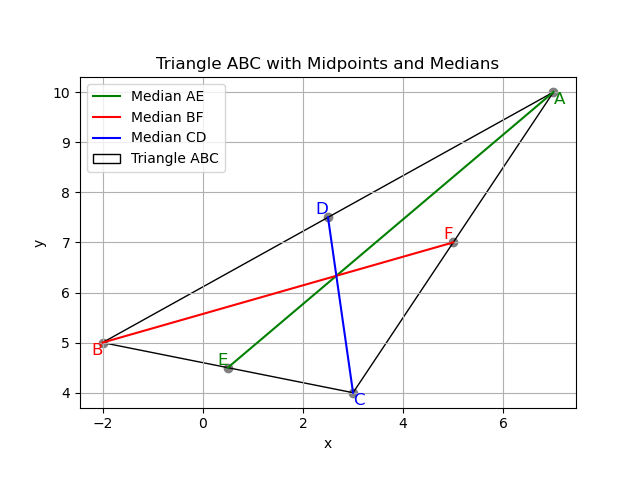
\includegraphics[width=0.5\linewidth]{figs/01.png}
   \caption{Plot of $\triangle$ABC}
   \label{Plot_1}
\end{figure}
\end{document}
